%TypeIIb.tex
\section{TypeII-b Example: 1987A}

Type II-P supernovae starkly contrast with the quick rise-and-drop in magnitude of other supernovae before $^{56}$Ni beta decay takes hold of the magnitude. Type II-L supernovae exhibit lightcurves very similar to those of Type Ias, but II-Ps show unusual slow rises and relatively flat plateaus that can stretch to 100 days or more \cite{nowakowski2018}. Here we plot magnitude versus time for five bands of 1987A, the quintessential Type II-P supernova, with special attention to its pre-plateau shape.

\begin{figure}[htp]
	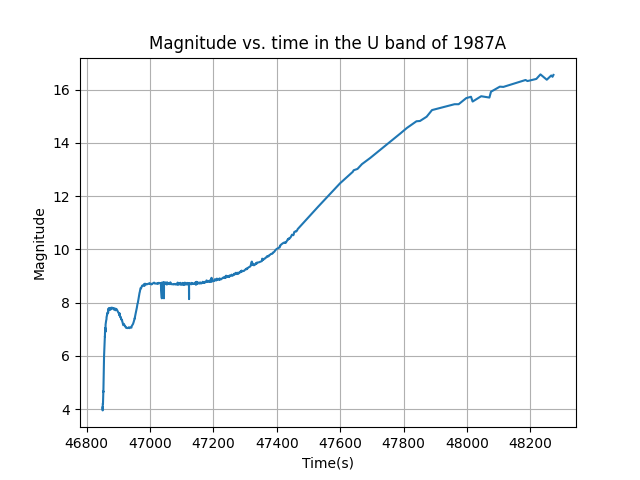
\includegraphics[width=0.5\textwidth]{1987A_U_magvstime.png}
	\caption{Change in brightness of SN1987A across time in the U band.}
\end{figure}
\begin{figure}[htp]
	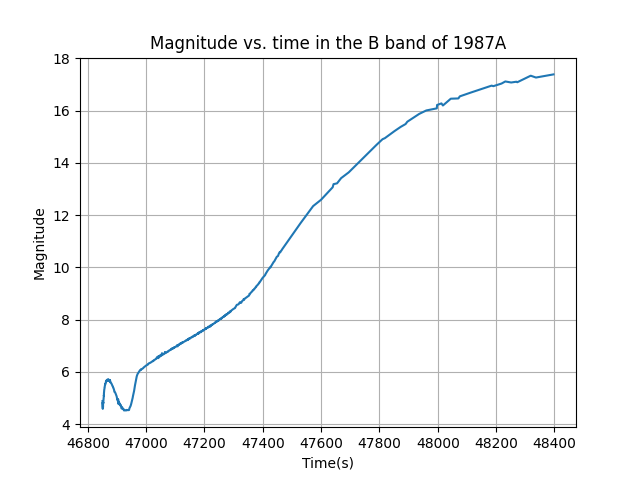
\includegraphics[width=0.5\textwidth]{1987A_B_magvstime.png}
	\caption{Change in brightness of SN1987A across time in the B band.}
\end{figure}
\begin{figure}[htp]
	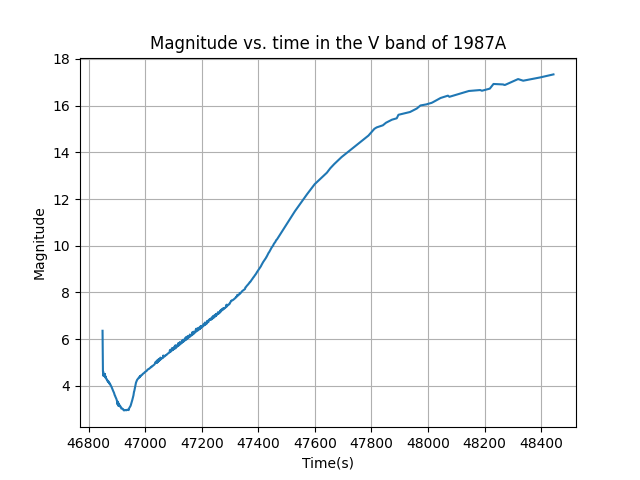
\includegraphics[width=0.5\textwidth]{1987A_V_magvstime.png}
	\caption{Change in brightness of SN1987A across time in the V band.}
\end{figure}
\begin{figure}[htp]
	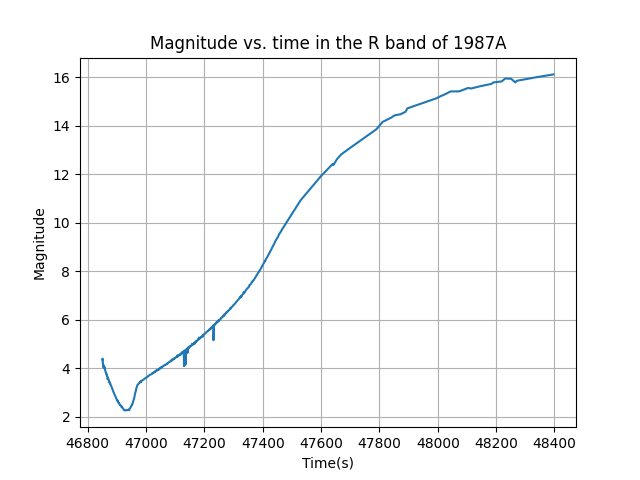
\includegraphics[width=0.5\textwidth]{1987A_R_magvstime.png}
	\caption{Change in brightness of SN1987A across time in the R band.}
\end{figure}
\begin{figure}[htp]
	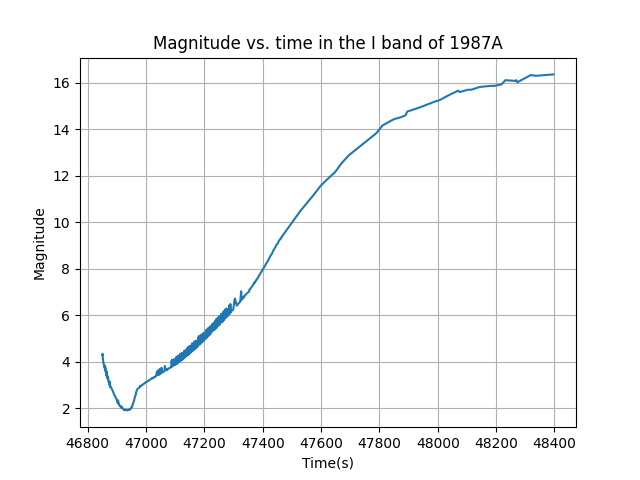
\includegraphics[width=0.5\textwidth]{1987A_I_magvstime.png}
	\caption{Change in brightness of SN1987A aross time in the I band.}
\end{figure}
\begin{figure}[htp]
	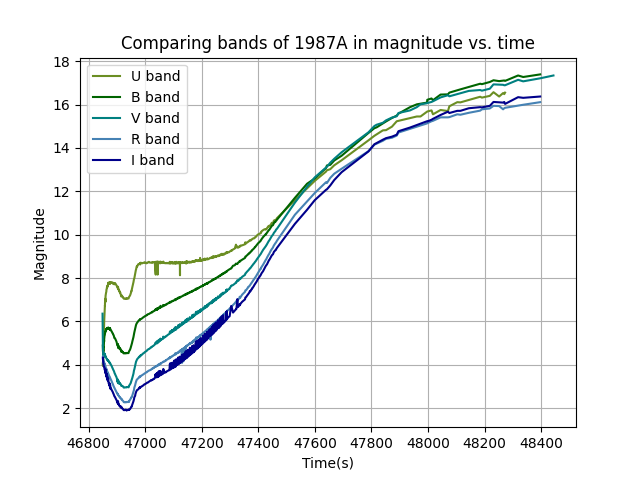
\includegraphics[width=0.5\textwidth]{1987A_all_magvstime.png}
	\caption{All bands of SN1987A together. Note the similarity in magnitude vs. time curve of each of the five bands, as opposed to the distinct differences between bands observed in 2014J.}
\end{figure}
